
\chapter{DL Figs}\label{chapter:DL_figs}


\begin{figure}[h!]
    \begin{minipage}{0.45\linewidth}
    \centering
    \begin{tikzpicture}
        %
        \def\Nnodes{9}
        \def\cellwidth{0.3}
        % draw xin
        \foreach \y in {1,...,\Nnodes} {
            \draw [fill=data_color] (\cellwidth,-\cellwidth*\y-0.5*\cellwidth) rectangle ++(\cellwidth,\cellwidth);
        }
        %
        \draw (\cellwidth*3,-\cellwidth) node {$=$};
        % draw W
        \foreach \x in {1,...,\Nnodes} {
            \foreach \y in {1,...,\Nnodes} {
                \draw [shift={(\cellwidth*3,0)}, fill=param_color] (\cellwidth*\x,-\cellwidth*\y-0.5*\cellwidth) rectangle ++(\cellwidth,\cellwidth);
            }
        }
        \draw (\cellwidth*8.5,-\cellwidth*5) node[scale=0.65, fill=param_color, draw=black, thick, text centered, minimum width=1cm] {$\mathbf{W}$};
        % draw xout
        \foreach \y in {1,...,\Nnodes} {
            \draw [shift={(\cellwidth*\Nnodes+\cellwidth*3.5,0)}, fill=data_color] (\cellwidth,-\cellwidth*\y-0.5*\cellwidth) rectangle ++(\cellwidth,\cellwidth);
        }
        %
        \draw (\cellwidth*1.5,-\cellwidth*\Nnodes-1.5*\cellwidth) node {$\xout$};
        \draw [shift={(\cellwidth*\Nnodes+\cellwidth*3.5,0)}] (\cellwidth*1.5,-\cellwidth*\Nnodes-1.5*\cellwidth) node {$\xin$};
        %
    \end{tikzpicture}
    \end{minipage}
    \begin{minipage}{0.08\linewidth}
    \centering
    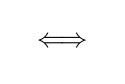
\begin{tikzpicture}
        \def\cellwidth{0.25}
        \def\Nnodes{9}
        \draw (0,-\cellwidth*0.5*\Nnodes) node {$\Longleftrightarrow$};
    \end{tikzpicture}
    \end{minipage}
    \begin{minipage}{0.45\linewidth}
    \centering
    \begin{tikzpicture}
        \begin{scope}[rotate=-90]
        %
        \def\Nnodes{9}
        \def\Nlayers{2}
        \def\layerheight{2.6}
        \def\neuronrad{0.14}
        \def\neuronstep{0.42}
        % draw all nodes
        \foreach \y in {1,...,\Nlayers} {
            \foreach \x in {1,...,\Nnodes} {
                \draw [fill=data_color] (\neuronstep*\x,\y*\layerheight-\layerheight) circle (\neuronrad);
            }
        }
        % draw nodes in RF
        % \node [circle, draw, inner sep=\neuronrad*0.7 cm, minimum size=\neuronrad, label=right:${\mathbf{x}_1[3]}$] (myNode) at (\neuronstep*4,\layerheight) {};
        %
        % draw all edges
        \pgfmathtruncatemacro{\NlayersMinusOne}{\Nlayers - 1}
        \pgfmathtruncatemacro{\NNodesPlusOne}{\Nnodes + 1}
        \foreach \y in {1,...,\NlayersMinusOne} {
            \foreach \x in {1,...,\Nnodes} {
                \foreach \k in {-1,...,1} {
                    \pgfmathtruncatemacro{\xk}{\x+\k}
                    \ifnum \xk>0
                    \ifnum \xk<\NNodesPlusOne
                        \draw [thin, color=black] [nn_edge] (\neuronstep*\x,\layerheight*\y+\neuronrad-\layerheight) -- (\neuronstep*\xk,\layerheight*\y-\neuronrad);
                    \fi
                    \fi
                }
            }
        }
        %
        \draw (\neuronstep*5,\layerheight*0.5) node[scale=0.65, fill=param_color, draw=black, thick, text centered, minimum width=1cm] {$\mathbf{W}$};
        %
        \draw (\neuronstep*\Nnodes+\neuronstep,0) node {$\xin$};
        \draw (\neuronstep*\Nnodes+\neuronstep,\layerheight) node {$\xout$};
        \end{scope}
    \end{tikzpicture}
    \end{minipage}
    \caption{Two equivalent visualizations of a convolutional layer.}
    \label{fig:convolutional_neural_nets:conv_matrix_vs_net}
\end{figure}



\begin{figure}[h!]
    \centerline{
    \begin{minipage}{0.49\linewidth}
    \centerline{
    \begin{tikzpicture}
        \begin{scope}[rotate=-90]
        %
        \def\Nnodes{7}
        \def\Nlayers{4}
        \def\layerheight{1.2}
        \def\neuronrad{0.1}
        \def\neuronstep{0.3}
        % draw all nodes
        \foreach \y in {1,...,\Nlayers} {
            \foreach \x in {1,...,\Nnodes} {
                \draw [fill=white] (\neuronstep*\x,\y*\layerheight-\layerheight) circle (\neuronrad);
            }
        }
        % draw nodes in RF
        \node [circle, draw, fill=black, inner sep=\neuronrad*0.7 cm, minimum size=\neuronrad, label=right:${x_2[3]}$] (myNode) at (\neuronstep*4,\layerheight*3) {};
        %
        \foreach \x in {3,...,5} {
            \draw [fill=black] (\neuronstep*\x,\layerheight*2) circle (\neuronrad);
        }
        %
        \foreach \x in {3,...,5} {
            \draw [fill=black] (\neuronstep*\x,\layerheight) circle (\neuronrad);
        }
        %
        \foreach \x in {2,...,6} {
            \draw [fill=black] (\neuronstep*\x,0) circle (\neuronrad);
        }
        % draw all edges
        \pgfmathtruncatemacro{\NlayersMinusOne}{\Nlayers - 1}
        \pgfmathtruncatemacro{\NNodesPlusOne}{\Nnodes + 1}
        \foreach \y in {1,...,\NlayersMinusOne} {
            \foreach \x in {1,...,\Nnodes} {
                \foreach \k in {-1,...,1} {
                    \pgfmathtruncatemacro{\isodd}{mod(\y,2)}
                    \ifnum\isodd=1
                        \foreach \k in {-1,...,1} {
                            \pgfmathtruncatemacro{\xk}{\x+\k}
                            \ifnum \xk>0
                            \ifnum \xk<\NNodesPlusOne
                                \draw [thin, color=gray!33] [nn_edge] (\neuronstep*\x,\layerheight*\y+\neuronrad-\layerheight) -- (\neuronstep*\xk,\layerheight*\y-\neuronrad);
                            \fi
                            \fi
                        }
                    \else
                        \draw [thin, color=gray!33] [nn_edge] (\neuronstep*\x,\layerheight*\y+\neuronrad-\layerheight) -- (\neuronstep*\x,\layerheight*\y-\neuronrad);
                    \fi
                }
            }
        }
        % draw edges in RF
        \foreach \k in {-1,...,1} {
            \pgfmathtruncatemacro{\xk}{4+\k}
            \draw [thick] [nn_edge] (\neuronstep*\xk,\layerheight*3+\neuronrad-\layerheight) -- (\neuronstep*4,\layerheight*3-\neuronrad);
        }
        \foreach \k in {-1,...,1} {
            \pgfmathtruncatemacro{\xk}{4+\k}
            \draw [thick] [nn_edge] (\neuronstep*\xk,\layerheight*2+\neuronrad-\layerheight) -- (\neuronstep*\xk,\layerheight*2-\neuronrad);
        }
        \foreach \kk in {-1,...,1} {
            \foreach \k in {-1,...,1} {
                \pgfmathtruncatemacro{\xkk}{4+\k+\kk}
                \pgfmathtruncatemacro{\xk}{4+\k}
                \draw [thick] [nn_edge] (\neuronstep*\xkk,\layerheight+\neuronrad-\layerheight) -- (\neuronstep*\xk,\layerheight-\neuronrad);
            }
        }
        % draw layer labels
        \draw (-0.2,\layerheight*0.5) node {\small \texttt{conv}};
        \draw (-0.2,\layerheight*1.5) node {\small \texttt{relu}};
        \draw (-0.2,\layerheight*2.5) node {\small \texttt{conv}};
        \end{scope}
    \end{tikzpicture}
    }
    \end{minipage}
    \begin{minipage}{0.49\linewidth}
    \centerline{
    \begin{tikzpicture}
        \begin{scope}[rotate=-90]
        %
        \def\Nnodes{7}
        \def\Nlayers{4}
        \def\layerheight{1.2}
        \def\neuronrad{0.1}
        \def\neuronstep{0.3}
        % draw all edges
        \pgfmathtruncatemacro{\NlayersMinusOne}{\Nlayers - 1}
        \pgfmathtruncatemacro{\NNodesPlusOne}{\Nnodes + 1}
        \foreach \y in {1,...,\NlayersMinusOne} {
            \foreach \x in {1,...,\Nnodes} {
                \foreach \k in {-1,...,1} {
                    \pgfmathtruncatemacro{\isodd}{mod(\y,2)}
                    \ifnum\isodd=1
                        \foreach \k in {-1,...,1} {
                            \pgfmathtruncatemacro{\xk}{\x+\k}
                            \ifnum \xk>0
                            \ifnum \xk<\NNodesPlusOne
                                \draw [thin, color=gray!33] [nn_edge] (\neuronstep*\x,\layerheight*\y+\neuronrad-\layerheight) -- (\neuronstep*\xk,\layerheight*\y-\neuronrad);
                            \fi
                            \fi
                        }
                    \else
                        \draw [thin, color=gray!33] [nn_edge] (\neuronstep*\x,\layerheight*\y+\neuronrad-\layerheight) -- (\neuronstep*\x,\layerheight*\y-\neuronrad);
                    \fi
                    }
            }
        }
        % draw all nodes
        \foreach \y in {1,...,\Nlayers} {
            \foreach \x in {1,...,\Nnodes} {
                \draw [fill=white] (\neuronstep*\x,\y*\layerheight-\layerheight) circle (\neuronrad);
            }
        }
        % draw layer labels
        \draw (-0.2,\layerheight*0.5) node {\small \texttt{conv}};
        \draw (-0.2,\layerheight*1.5) node {\small \texttt{relu}};
        \draw (-0.2,\layerheight*2.5) node {\small \texttt{conv}};
        \end{scope}
    \end{tikzpicture}
    }
    \end{minipage}
    }
    \caption{Receptive fields in a CNN. The black filled neurons are within the receptive fields of each labeled neuron (left: ${x_2[3]}$, right: ${x_1[5]}$).}
    \label{fig:convolutional_neural_networks:RFs}
\end{figure}